\chapter{Redes Neurais}
\label{chap:neuro}

\begin{epigraphs}
\qitem{One of the great intellectual challenges for the next few
decades is the question of brain organization. What is the basic mechanism
for storage of memory? What are the processes that serve as the interface
between the basically chemical processes of the body and the very specific
and non-statistical operations of the brain? Above all, how is concept
formation achieved in the human brain? I wonder whether the spirit of the
physics that will be involved in these studies will not be akin to that which
moved the founders of the "rational foundation of thermodynamics". } 
{\----\textsc{C.N. Yang, 1922- }}
\end{epigraphs}


O neurônio, de forma extremamente simplificada, pode ter seu funcionamento
descrito como uma série de impulsos elétricos que são recebidos pelas
partes de sua célula chamadas de dendritos. Por eles, os impulsos são
enviados para o corpo da célula, sendo que durante o envio os impulsos
podem ser atenuados ou amplificados, a depender do dendrito. A combinação
desses impulsos é recebida pelo corpo célular, que modifica esses sinais
de alguma maneira e os envia na forma de pulsos através do axônio. Estes
pulsos se propagam até as terminações nervosas do axônio, de onde são
transmitidos para dendritos de outros neurônios.
\begin{marginfigure}
    \centering
    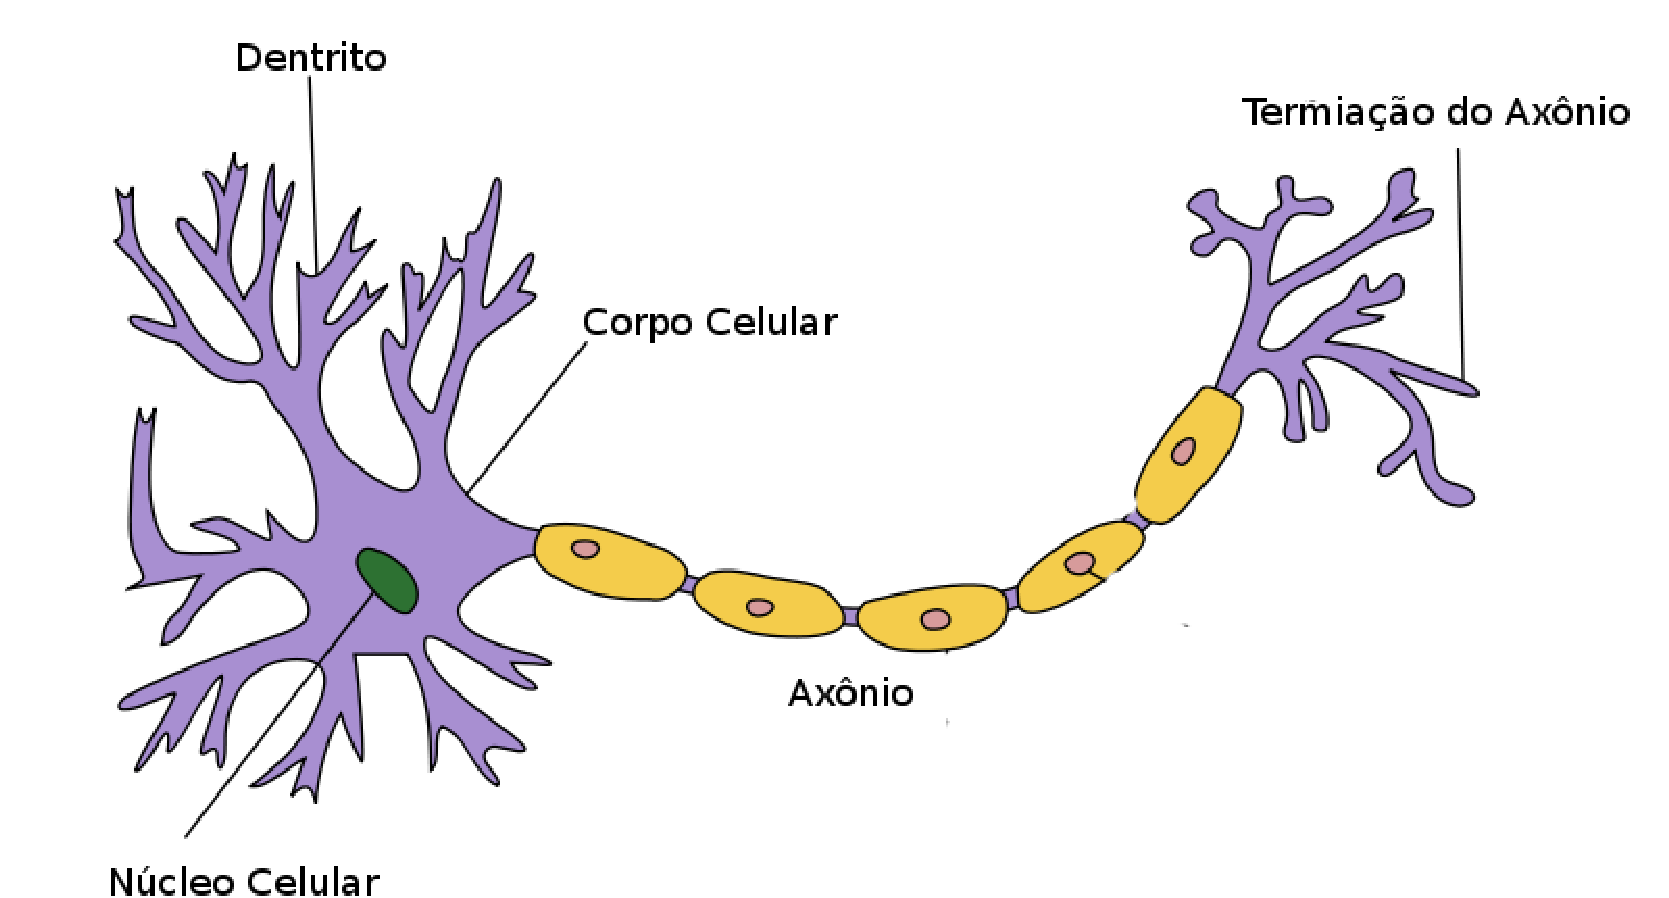
\includegraphics[scale = 0.2]{Figures/neuronio}
    \caption{Ilustração de um neuronio retirada de \citep{NeuronWiki}}
\end{marginfigure}

É claro que biologicamente esse processo é muito mais complexo, sendo
esses impulsos causados por trocas de íons que têm suas taxas controladas
por vários fatores. No entanto, esse esquema de funcionamento do neurônio
serve de inspiração para o modelo matemático de rede neural que iremos
usar. Dentre as várias descrições matemáticas do neurônio, a mais
simples é a descrição do \textbf{perceptron}, introduzida por Rosenblatt
no final da decada de 1950 \citep{Rosenblatt1958}. Por essa descrição,
representaremos os impulsos que chegam ao axônio como um vetor  de
$N-$dimensões $\mathbf{X} = \left( X_1, X_2, \cdots, X_N   \right) $. Esse
impulso de entrada é ponderado por um vetor de pesos sinápticos $\mathbf{J}
= \left( J_1,J_2,\cdots,J_N\right)$ de mesma dimensão.  O impulso de saída é
modelado como uma função desses dois vetores, $ f\left(\mathbf{X},\mathbf{J}
\right) $.

\begin{marginfigure}
    \centering
    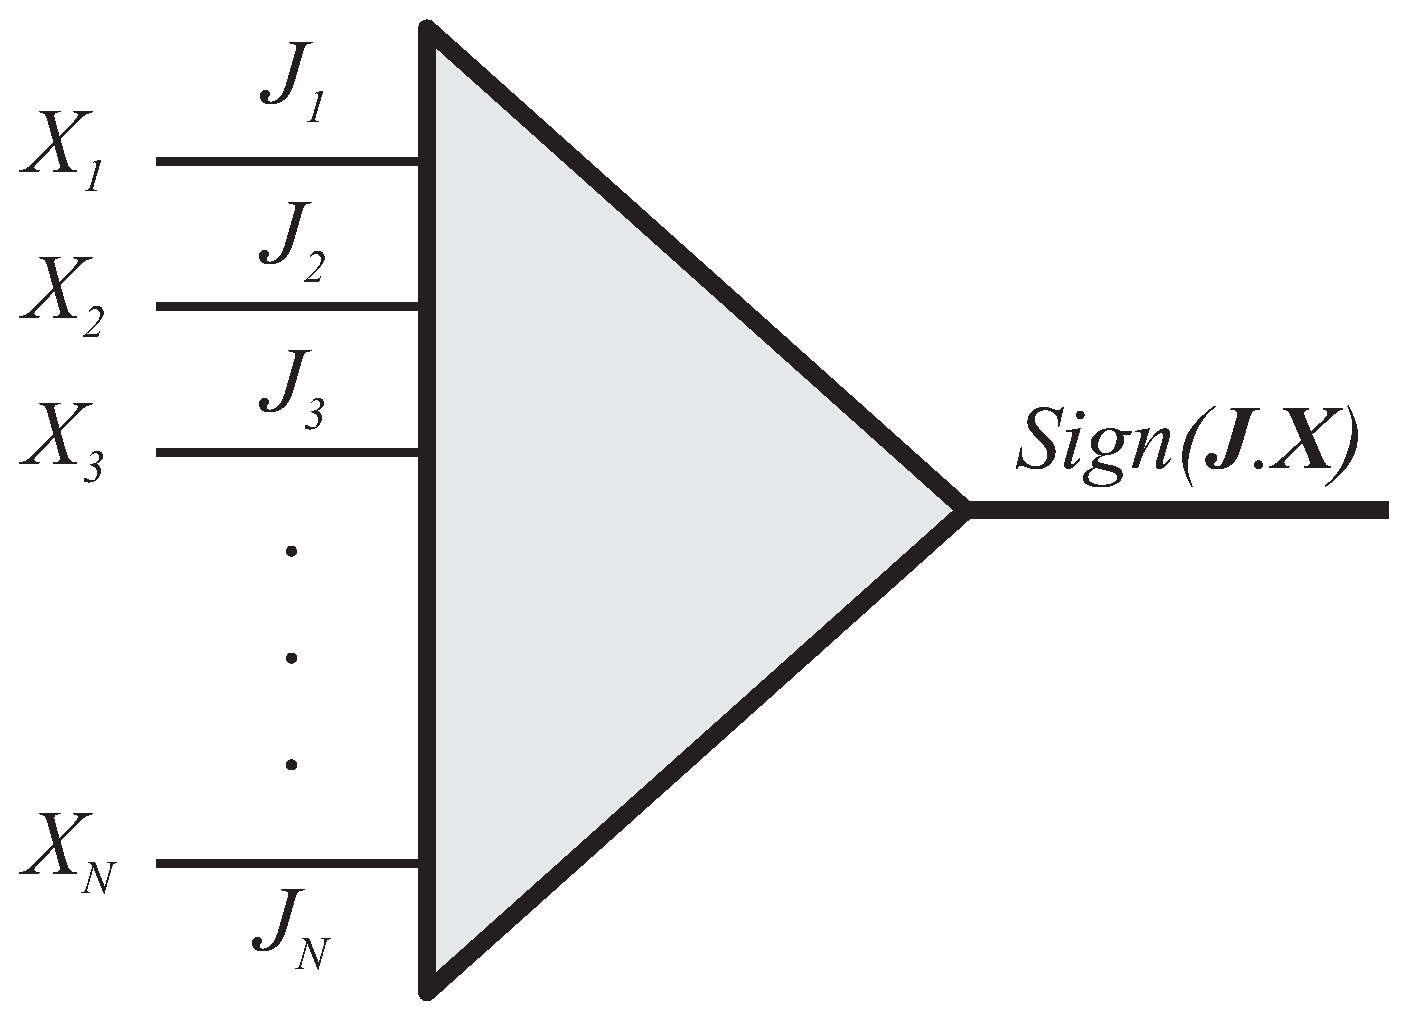
\includegraphics[scale = 0.15]{Figures/circuitogay}
    \caption{Representação matemática de uma rede neural}
\end{marginfigure}

Faremos ainda uma descrição mais simplista do neurônio \citep{Engel2004},
fazendo com que o perceptron seja basicamente um classificador booleano
do vetor de entrada $\mathbf{X} \in \mathbb{R}^N$,  onde $ f \left(
\mathbf{J}\cdot\mathbf{X} \right) = \sigma\left[\mathbf{J},\mathbf{X}\right]=
Sign\left(\mathbf{J}\mathbf{X}\right)$. Assim, o perceptron separa os vetores
de entrada em dois hiperplanos, um que está na direção do perceptron
e outro na direção contrária.


\section{ Perceptron Booleano }

O modelo de rede neural do perceptron, apesar de simples, é muito útil
para lidar com problemas em que existe uma classificação linear de dados.
Dentre os vários tipos de algoritmos de aprendizado para redes neurais,
um dos mais conhecidos são os algoritmos de aprendizado supervisionado
do perceptron. Nesses algoritmos, vetores de entrada (que chamaremos de
assuntos), provindos de uma distribuição de probabilidade $P_0(\mathbf{X})$,
são apresentados juntamente com uma classificação pré-estabelecida $
(\mathbf{X}_\mu, \sigma_\mu )$, sendo $\mu = 1,\ldots,p$. O algoritmo de
aprendizado fará com que o perceptron, usando essa informação, mude seus
pesos sinápticos $\mathbf{J}$ a fim de que sua classificação coincida
com a classificação pré-estabelecida dos assuntos.

Existem dois paradigmas de aprendizado para o perceptron \cite{Engel2004},
o aprendizado on-line e aprendizado off-line. No aprendizado off-line ou
aprendizado de Gibbs, a direção do perceptron é encontrada usando todos
os exemplos de uma vez. Neste texto, nos restringiremos apenas na discussão
dos algoritmos de aprendizado on-line, já que esse pode ser interpretado mais
facilmente sobre a perspectiva de aprendizado por reforço. Nele, um perceptron
$\mathbf{J}$, ao qual chamaremos de \textbf{estudante} muda a direção
de seus pesos sinápticos de acordo com a equação \eqref{eq:aprend1}
\begin{equation}
  \mathbf{J}_{\mu +1} = \mathbf{J}_\mu - \frac{1}{N}\nabla_\mathbf{J}V_\mu ,
  \label{eq:aprend1}
\end{equation}
onde $ \nabla_\mathbf{J}V_\mu \equiv -\mathit{W}_\mu\sigma_B^\mu\mathbf{X}_\mu$
por definição. O índice $\mu=1,\ldots,p$ indica o tempo de
treinamento do algoritmo. A classificação \textit{a priori} do
assunto é provida por um outro perceptron $\mathbf{B},$ chamado de
\textbf{professor}, através do sinal do produto escalar com o professor,
$\sigma_B^\mu=sign\left(\mathbf{B}.\mathbf{X}_\mu\right)$.

Com isso, vemos que o perceptron aluno muda nos seus pesos sinápticos
na direção $\sigma_B^\mu \mathbf{X}$, conhecido como
termo Hebbiano. O fator de proporcionalidade$ W_\mu$ é chamado de
função de modulação. É esperado que, após um tempo de treinamento
suficientemente longo, o aluno classifique os assuntos

\begin{figure}
    \centering
    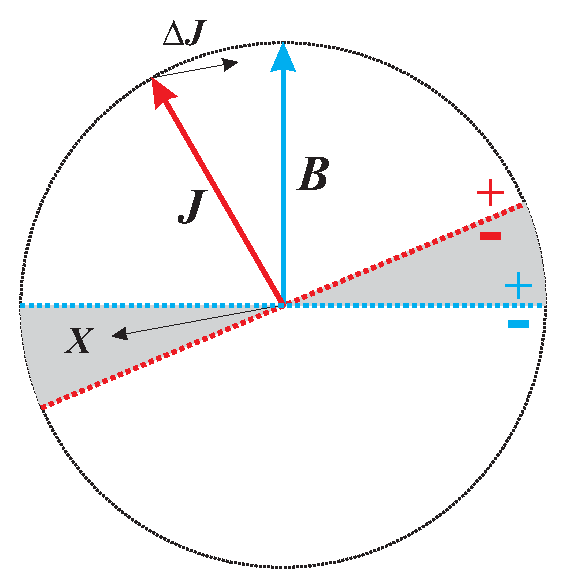
\includegraphics[scale = 0.6]{Figures/bolinhagay}
    \caption{\textit{Representação do hiperplano do perceptron e do
    algoritmo de aprendizado}. O vetor exemplo $\mathbf{X}$ é classificado
    pelos perceptrons professor $\mathbf{B}$ e aluno $\mathbf{J}$, em $+1$
    ou $-1$, dependendo de que lado do hiperplano de cada um o vetor se
    encontra. Na região escura os vetores de exemplo são classificados
    diferentemente por professor e aluno. O vetor $\Delta \mathbf{J}$ é
    a correção (proporcional ao termo hebbiano $\sigma_B\mathbf{X}$) na
    direção do aluno.}
\end{figure}

Existem vários tipos de função de regulação $ W_\mu$ estudadas na
literatura, quando $ W=1 $ temos o algoritmo de aprendizado Hebbiano. O
algoritmo do perceptron propriamente dito é tido quando $W_\mu = \Theta\left(
- h_\mu \sigma_\mathbf{B}\right)$, sendo $\Theta\left(x\right)$ a função
degrau de Heaviside 
\footnote{ A função de Heaviside é dada por,
\begin{equation}
  \Theta\left(x\right)=\left\{
  \begin{array}{c}
    1 \quad se \quad x\geq 0,  \\
    0 \quad se \quad x<0. 
  \end{array} 
  \right.
\end{equation} 
}, onde 
\begin{equation}
  h = \frac{\mathbf{J}\cdot\mathbf{X}^\mu}{ \left|\mathbf{J}\right|} \qquad
  \text{e}  \qquad b = \mathbf{B}\cdot\mathbf{X}^\mu.
\end{equation}

Diferentemente do algoritmo de aprendizado hebbiano, que sempre muda o vetor
de pesos sinápticos do estudante, o algoritmo do perceptron estudante só
muda os pesos sinápticos quando ele discorda do professor. O potencial de
aprendizado do algoritmo de Hebb é $ V_\mu = -h_\mu\sigma_B$ e o potencial do
algoritmo do perceptron é $V_\mu = -h_\mu\sigma_B\Theta\left(-h_\mu\sigma_B\right)$.

A medida natural de quanto o aluno está alinhado com o professor é conhecida
como \textit{overlap} $\rho$ que é simplesmente o produto escalar entre os
vetores sinápticos do professor e do aluno dividido por suas normas. 
\begin{equation}
  \rho =
  \frac{\mathbf{B}\cdot\mathbf{J}}{\left|\mathbf{B}\right|\left|\mathbf{J}\right|}.
  \label{eq:def_rho}
\end{equation}

Na próxima seção veremos que a variação de $\rho$ em relação ao tempo
de treinamento está diretamente relacionada com a eficiência do algoritmo
de aprendizado para diferentes funções de modulação.

\section{Aprendizado Ótimo}
\label{sec:AprendizadoOtimo}

Uma ferramenta útil para medirmos a convergência do algoritmo
aprendizado do perceptron é o \textbf{erro de generalização}
\cited{Kinouchi1992,Vicente1998} que é definido como a média, sobre a
distribuição de assuntos, dos erros instantâneos
\[
 e_P = \frac{1}{2}\left(
1 - \sigma_J\sigma_B \right)= \frac{1}{2}\Theta\left(-hb\right). 
\]
Em outras palavras, o erro de generalização é a probabilidade de que o
estudante classifique um assunto aleatório da mesma maneira que o professor,
\begin{align}
    e_G 
    &= 
    \int\dd\mathbf{X} P_0\left( \mathbf{X} \right) e_P 
    \left[ 
        \sigma_J\left( \mathbf{X} \right) \sigma_B \left( \mathbf{X} \right)
    \right],
    \nn
    &= 
    \int \dd \mathbf{X} P_0\left( \mathbf{X} \right) \frac{1}{2}
    \Theta\left[ -\left(\mathbf{J}\cdot\mathbf{X}\right)
    \left( \mathbf{B}\cdot\mathbf{X}\right) \right].
    \label{eq:erro_X}
\end{align}
No \textit{Limite Termodinâmico}, que acontece quando $N \rightarrow \infty$,
podemos provar que o erro de generalização depende exclusivamente do overlap
entre o estudante e o aluno  $\rho$, de acordo com a seguinte expressão,
 \cite{Engel2004}.
\begin{align}
    e_G 
    &= \int \dd h \dd b P \left(h,b\right) \Theta \left( -hb \right)\nn 
    &= \frac{1}{\pi}\cos^{-1}\left( \rho \right) 
    \label{eq:rho_cos}
\end{align}
Nesse limite, pode-se provar, usando o \textit{Teorema Central
do Limite}, que a distribuição $P\left(h,b\right)$ é uma distribuição
normal de média nula e matriz de correlação dada por
\begin{equation}
  C = \left( 
  \begin{array}{cc} 
    1 & \rho \\
    \rho & 1
  \end{array}
  \right),
\end{equation}
onde a correlação $\rho$ entre o estudante e professor é exatamente
overlap definido em \eqref{eq:def_rho}. De forma explícita,
a distribuição de probabilidade dos assuntos em relação ao perceptron
estudante e professor é
\begin{equation}
  P\left(h,b\right) = \frac{1}{2\pi\sqrt{1 - \rho^2}}
  \exp  -\frac{ h^2 - 2 \rho h b + b^2 }{ 2\left( 1 -\rho^2 \right) }.
\end{equation}

O nosso objetivo é encontrar uma função de modulação $W_\mu$
que faça com que o perceptron aprenda com o menor número de exemplos
possíveis. Introduzindo as variáveis, $J_\mu = \left|\mathbf{J}_\mu\right|$
e $R_\mu = \mathbf{J}_\mu\cdot\mathbf{B}$ e lembrando que a equação de
aprendizado é dada por,
\begin{equation}
  \mathbf{J}_{\mu+1} = 
  \mathbf{J}_\mu  + \frac{1}{N}\mathit{W}_\mu\sigma_B\mathbf{X}_\mu,
  \label{eq:Jmu}
\end{equation}
segue que a dinâmica dessas variáveis é descrita por,
\begin{align}
    R_{\mu +1} &=   
    R_\mu  + \frac{1}{N}\mathit{W}_\mu\sigma_B^\mu b_\mu  
    \label{eq:evolve_R}; \\
    J_{\mu+1} &=  
    J_\mu \left[ 1 + \frac{1}{N} 
        \left( 2 \frac{\mathit{W}_\mu}{J_\mu} \sigma_B^\mu h_\mu 
    + \frac{\mathit{W}_\mu^2}{J_\mu^2} \right) \right]^{1/2}; \nn 
    &\approx  J_\mu \left[ 1 + \frac{1}{N}
    \left( \frac{\mathit{W}_\mu}{J_\mu} \sigma_B^\mu h_\mu + 
\frac{\mathit{W}_\mu^2}{2J_\mu^2} \right) \right] 
\label{eq:evolve_J};
\end{align}
onde consideramos $\left|X_\mu\right| \propto
\mathcal{O}\left(N\right) $ e desprezamos termos de ordem superior á $1/N$.
Com isso, podemos escrever a evolução do overlap entre aluno e
professor como,
\begin{align}
    \rho_{\mu+1} &= \frac{ R_{\mu+1} }{ J_{\mu+1} }, \nonumber\\ 
                 &=  \frac{R_\mu  + \mathit{W}_\mu\sigma_B^\mu b_\mu}
    {{J_\mu \left[ 1 + \frac{1}{N}
                \left( 2 \frac{\mathit{W}_\mu}{J_\mu} \sigma_B^\mu h_\mu 
    + \frac{\mathit{W}_\mu^2}{J_\mu^2} \right) \right]^{1/2}} };\nn 
    &\approx \rho_\mu + \frac{1}{N}\left[ \left( 
    b_\mu -\rho_\mu h_\mu \right)\sigma_B^\mu\frac{\mathit{W}_\mu}{J_\mu} 
- \frac{\rho_\mu \mathit{W}_\mu^2}{2J_\mu^2} \right].
\label{eq:evolve_rho}
\end{align}
As equações \eqref{eq:evolve_R} e \eqref{eq:evolve_J} são estocásticas,
elas  podem ser escritas como equações diferenciais no Limite Termodinâmico
ao definirmos $\alpha = \mu/N$, de onde teremos $\dd \alpha = 1/N$,
\begin{align}
  \frac{\dd R}{\dd \alpha} &=  \mean{\mathit{W}\sigma_B b},  \label{eq:dif_R}\\
  \frac{\dd J}{\dd \alpha} &= J\mean{ \frac{\mathit{W}}{J} \sigma_B h 
    + \frac{\mathit{W}^2}{2J^2} }; \label{eq:dif_J}\\    
  \frac{\dd \rho}{\dd \alpha} &= 
    \mean{ \left( b -\rho h \right)\sigma_B\frac{\mathit{W}}{J} 
    - \rho \frac{\mathit{W}^2}{2J^2} }; \label{eq:dif_rho}
\end{align}
onde $\mean{\cdots} = \int \dd\mathbf{X} P_0 \left( \mathbf{X}
\right)\left[\cdots\right] $ é a média tomada sobre a distribuição
de exemplos.

Para maximizarmos a taxa de aprendizado do algorítimo devemos
minimizar a taxa do erro de generalização. A ideia do algorítimo de
aprendizado ótimo\cite{Kinouchi1992}, vem do fato que o erro de generalização
é função exclusiva do overlap entre o professor e o aluno, e esse é um
funcional da função de modulação, de onde segue,
\[ 
    \frac{\dd e_G}{ \dd \alpha}\left[W\right]
        = \frac{\dd e_G}{ \dd \rho}\frac{\dd \rho}{ \dd \alpha}\left[W\right]
\]

Cada função de modulação $\mathit{W}$ leva a uma dinâmica de aprendizado
diferente, então, podemos fazer uma derivada funcional de overlap em relação à
função de modulação para encontrarmos uma função que minimiza o tempo
de aprendizado,
\begin{equation}
  \frac{\delta}{\delta \mathit{W}} \left[ \frac{\dd \rho}{ \dd \alpha} \right] 
  = 0. 
  \label{eq:dif_W}
\end{equation}

Portanto, a partir de  \eqref{eq:dif_rho} e \eqref{eq:dif_W} 
encontramos que a função que minimiza o tempo de aprendizado é dada por
\begin{equation}
  \mathit{W}_\mu^* = J_\mu \left( \kappa_\mu -z_\mu \right),
  \label{eq:opt1}
\end{equation}
com
\begin{equation}
  \kappa_\mu = \frac{\sigma_B^\mu b_\mu}{\rho_\mu} 
  \qquad \text{e} \qquad z_\mu = \sigma_B^\mu h_\mu .
\end{equation}

Percebemos que a função de aprendizado ótima escrita na forma
\eqref{eq:opt1} depende de dois tipo de variáveis:
\begin{description}
  \item \textbf{Visiveis}: Que são as variáveis que o estudantes tem acesso, 
   \[  
       \mathcal{V} = \{h_\mu , \sigma_B^\mu \}
   \]
  \item \textbf{Invisiveis}: Que são as variáveis que o estudante não tem
      acesso,
      \[
          \mathcal{H} = \{ \left|b_\mu\right| \}
      \]
\end{description}

O algorítmo de aprendizado ótimo será realista somente se a função
de modulação $\mathit{W}^*$ for calculada tomando-se a média sobre
as variáveis invisíveis dado o conhecimento das visíveis.  Com isso,
a função de modulação ótima será dada por,
\begin{equation}
  \bar{\mathit{W}}= \mean{\mathit{W}^*}_{\mathcal{H}\left|\mathcal{V}\right.},
  \label{eq:W_mean}
\end{equation} 
onde $\mean{\cdots}_{\mathcal{H}\left|\mathcal{V}\right.}
= \int \dd \mathcal{H} P \left(\mathcal{H}\left|
\mathcal{V}\right. \right)\left[\cdots\right]$. 

Sabendo que a distribuição de probabilidade conjunta das variáveis
visíveis e invisíveis é dada por, $P\left(\mathcal{H},\mathcal{V}\right)=
P\left(\mathcal{H}\right)P\left(\mathcal{H}\left|\mathcal{V}\right.\right)$
e lembrando da regra de Bayes, 
\begin{equation}
  P \left(\mathcal{H}\left| \mathcal{V}\right. \right) 
  = \frac{P \left(\mathcal{H},\mathcal{V} \right)}
  { \int \dd \mathcal{H} P \left(\mathcal{H},\mathcal{V}\right)},
  \label{eq:BayesHV}
\end{equation}
podemos ver que a função de modulação ótima deve ser calculada pela integral
\begin{equation}
  \mathit{\bar{W}} = \frac{\int \dd \left|b\right| P \left( b, h \right) 
  \mathit{W}^* }{\int \dd \left|b\right| P \left( b, h \right)}.
  \label{eq:W_int}
\end{equation}
Essa integral  é calculada mais facilmente vendo que
\[
\int \dd \left|b\right| \left[\cdots \right] =
\int \dd b  \left[\Theta\left( b\right) - \Theta\left(-b\right) \right]
\left[\cdots \right].
\]
Logo a expressão para função de modulação do aprendizado ótimo é 
\begin{equation}
  \mathit{W}\left( \rho_\mu, J_\mu, z_\mu \right) 
  = \frac{1}{\sqrt{2\pi}}J_\mu \lambda_\mu 
  \exp\left(-\frac{z_\mu^2}{2\lambda_\mu^2} \right) 
  \frac{1}{H\left( - z_\mu/ \lambda_\mu \right)},
  \label{eq:W_final} 
\end{equation}
onde 
\begin{equation}
  \lambda = \tan\left(\pi e_g\right) = \frac{\sqrt{1- \rho^2 }}{ \rho}
  \label{eq:lamb}
\end{equation}
e
\begin{equation}
  H\left(x\right) = \frac{1}{2\pi}\int_x^\infty \dd y \exp(\frac{-y^2}{2}) 
  = \frac{1}{2}\mathrm{ercf}\left( \frac{x}{\sqrt{2}}\right)
\label{eq:ferr}
\end{equation}

Na figura \ref{fig:fmod} da sessão \ref{sec:fmod},  representamos a curva da
função de aprendizado para alguns valores de $\rho$ com o tamanho do vetor
aluno fixo em $J =1$ em função de $z$. Podemos perceber, que quanto mais
o vetor aluno aprende, ou seja, quanto maior o valor de $\rho$, mais o aluno
aprende com os exemplos que ele classifica de maneira diferente do professor
( $z < 0$ ) em comparação com os exemplos que ele classifica do mesmo modo
( $z>0$ ).


%Além disso, podemos 

